\section{Mechanical Equilibrium}

in this chapter, we will study the mechanical equilibrium of objects

for \emph{point objects}, zero resultant force suffices for equilibrium

but for \emph{rigid bodies}, force many produce \emph{turning effects}

hence rigid bodies must satisfy another condition to stay in equilibrium

this brings forward the notion of moment of a force and the principle of moments


\subsection{moment of force}

\begin{ilight}
	\keypoint{torque}\index{torque}, or \keypoint{moment}\index{moment} of a force, is defined as the product of the force and the perpendicular distance from the pivot to the line of action: $ \boxed{\tau = Fd_\perp} $
\end{ilight}

\begin{wrapfigure}{r}{0.44\textwidth}
	\vspace*{-5pt}
	\centering
	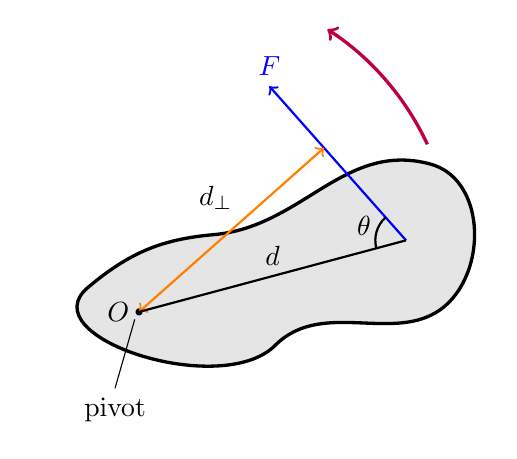
\begin{tikzpicture}[scale=0.78,rotate=15]
	\draw[fill=gray!20,very thick] (-3.2,0.4) to [out=25,in=170] (-1,0.7) to [out=-10,in=150] (2.7,0.9) to [out=-30,in=35] (2.5,-1.3) to [out=215,in=30] (-0.5,-1.3) to [out=210,in=205] (-3.2,0.4);
	\draw[thick,blue,->] (2,-.2) --++ (-1.5,3) node[above]{$F$};
	\draw[fill] (-2.5,-.2) circle (0.05) node[left]{$O$};
	\draw (-2.6,-.3) --++ (-.6,-1) node[below]{pivot};
	\draw[thick,orange,<->] (-2.5,-.2) --++ (26.565:4.025) node[pos=0.56,above left,black]{$d_\perp$};
	\draw[thick] (-2.5,-.2) -- (2,-.2) node[midway,above]{$d$};
	\draw[thick] (1.5,-.2) arc(180:116.565:.5);
	\node at (1.4,0.2) {$\theta$};
	\draw[very thick,purple,->] (24:3) arc(10:42:4.5);
	\end{tikzpicture}
	\vspace*{-16pt}
\end{wrapfigure}

\cmt unit of torque/moment: $[\tau] = \text{N m}$

\cmt perpendicular distance from pivot to the line of action is also called the \keypoint{lever arm}\index{lever arm}

this is the shortest distance between the force applied and axis of rotation

in the diagram, lever arm $d_\perp = d\sin\theta$

so moment of this force is: $\tau = Fd\sin\theta$

\cmt moment is a vector quantity
\footnote{Using vector notation, moment of a force can be defined as a \emph{cross product}: $\overrightarrow{\tau} = \overrightarrow{r}\times\overrightarrow{F}$, where $\overrightarrow{r}$ is the position vector from the pivot to the point at which the force is applied.}
\footnote{Rigorously speaking, moment is a \emph{pseudovector}, which means that it does not transform quite like a normal vector although it does have a direction. In particular, if an object acted by a force is reflected across a plane, the moment of this force would not be reflected. Instead, it would be reflected and \emph{reversed}.}

it can act in \emph{clockwise} or \emph{anti-clockwise} direction

\cmt moment of a force produces turning effects\footnote{Moment is like the rotational counterpart of a force: force changes the state of translational motion, moment changes the state of rotation.}

if there exists a non-zero moment, the object will start to rotate clockwise or anti-clockwise

\cmt note that moment of a force depends on choice of pivot

moment of the same force with respect to different points can be very different



\subsubsection{torque of couple}\label{ch:torque-of-couple}

let's take a pair of equal but opposite forces acting at different positions on the same object

\begin{wrapfigure}{r}{0.33\textwidth}
	\centering
	\vspace*{-8pt}
	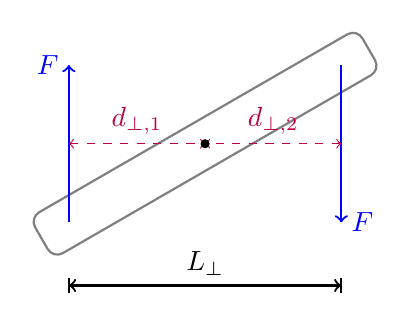
\begin{tikzpicture}
	\draw[thick,gray, rotate=30, rounded corners] (-2.4,-.3) rectangle (2.4,.3);
	\draw[thick,blue,->] (-1.73,-1) -- ++(0,2) node[left]{$F$};
	\draw[thick,blue,->] (1.73,1) -- ++(0,-2) node[right]{$F$};
	\draw[dashed,<->,purple] (-1.73,0) -- (0,0) node[midway,above]{$d_{\perp,1}$};
	\draw[dashed,<->,purple] (1.73,0) -- (0,0) node[midway,above]{$d_{\perp,2}$};
	\draw[fill] (0,0) circle(0.05);
	\draw[thick,<->] (-1.73,-1.8) -- (1.73,-1.8) node[midway,above]{$L_\perp$};
	\draw[thick] (-1.73,-1.9) -- (-1.73,-1.7) (1.73,-1.9) -- (1.73,-1.7);
	\end{tikzpicture}
	\vspace*{-16pt}
\end{wrapfigure}

the two forces produce torques in the same direction

the combined effect is called the torque of a couple



resultant torque due to the couple is

{
	\centering
	
	$ \tau = Fd_{\perp,1} + Fd_{\perp,2} = 2F(d_{\perp,1} + d_{\perp,2}) $
	
}

$d_{\perp,1} + d_{\perp,2}$ is perpendicular distance $L_\perp$ between the pair, so

{
	\centering
	
	$ \boxed{\tau = F L_\perp} $
	
}

\begin{ilight}
	\keypoint{torque of a couple} can be therefore defined as the product of one force in the couple and the perpendicular distance between the pair
\end{ilight}

\cmt a pair of equal but opposite forces give zero net force

but they can produce rotational effects, so no net force does not necessarily mean equilibrium

\cmt torque of couple does not depend on choice of pivot

for same force pair, resultant moment is constant about any point



\subsubsection{moment of weight}

recall that weight is a force of gravity which is actually experienced by every part of the object

when dealing with moment of weight, we need to sum up torques on each part of this object

this brings a problem since the lever arms can be all different

fortunately, this calculation can be simplified using the idea of centre of gravity

\begin{ilight}
	\keypoint{centre of gravity} is a point at which the entire weight of an object is considered to act
\end{ilight}

\cmt there is a similar concept called the centre of mass

\keypoint{centre of mass} is the average position of all the mass that makes up the object

near the surface of the earth, mass and weight are directly proportional to each other

so centre of mass is interchangeable with centre of gravity if we stay on earth

\cmt for a regularly-shaped uniform object, the centre of gravity/mass is its geometrical centre

\cmt if an object is hung freely, centre of gravity/mass is vertically below the point of suspension

otherwise weight would produce a non-zero torque about the point of suspension, causing the object to rotate until torque becomes zero

\begin{figure}[ht]
	\centering
	\begin{minipage}[b]{0.45\textwidth}
		\centering
		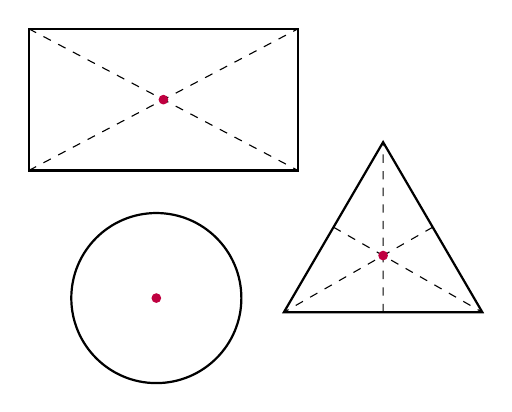
\begin{tikzpicture}[scale=0.9]
		% triangle
		\draw[thick] (-1.4,0) -- (0,2.4) -- (1.4,0) --cycle;
		\draw[dashed] (0,0) -- (0,2.4) (0.7,1.2) -- (-1.4,0) (-0.7,1.2) -- (1.4,0);
		\draw[purple,fill] (0,0.8) circle (0.06);
		% rectangle
		\draw[thick] (-5,2) rectangle (-1.2,4);
		\draw[dashed] (-5,2) -- (-1.2,4) (-5,4) -- (-1.2,2);
		\draw[purple,fill] (-3.1,3) circle (0.06);	
		% circle
		\draw[thick] (-3.2,0.2) circle(1.2);
		\draw[purple,fill] (-3.2,0.2) circle (0.06);		
		\end{tikzpicture}
		
		
		centre of mass of uniform lamina
		
		is at the geometrical centre
	\end{minipage}\hfil
	\begin{minipage}[b]{0.45\textwidth}
		\centering
		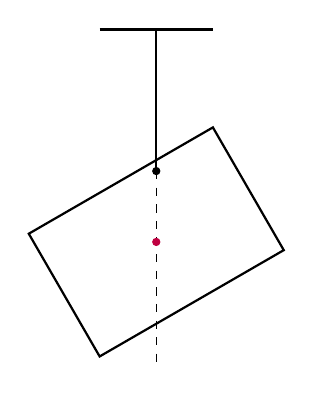
\begin{tikzpicture}[scale=0.9]
		\draw[thick,rotate=30] (-1.5,-1) rectangle (1.5,1);
		\draw[fill] (0,1) circle (0.05);
		\draw[thick] (0,1) -- (0,3);
		\draw[very thick] (-0.8,3) -- (0.8,3);
		\draw[dashed] (0,1) -- (0,-1.8);
		\draw[purple, fill] (0,0) circle (0.05);
		\end{tikzpicture}
		
		centre of mass is vertically below
		
		the point of suspension
	\end{minipage}
\end{figure}

\cmt to find the centre of gravity/mass, the object of interest is suspended from several positions

each time we draw a plumb-line through the point of suspension

centre of mass/gravity lies where the lines intersect


\begin{wrapfigure}{r}{0.45\textwidth}
	\vspace*{-8pt}
	\centering
	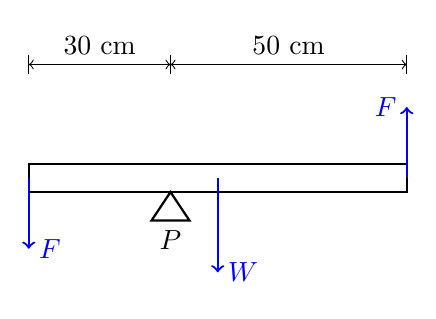
\begin{tikzpicture}[scale=0.6]
	\draw[thick] (-4,-.3) rectangle (4,.3);
	\draw[thick] (-1,-.3) --++ (.4,-.6) --++ (-.8,0) node[midway,below]{$P$} -- cycle;
	\draw[thick,blue,->] (0,0) -- (0,-2) node[right]{$W$};
	\draw[thick,blue,->] (4,0) --++ (0,1.5) node[left]{$F$};
	\draw[thick,blue,->] (-4,0) --++ (0,-1.5) node[right]{$F$};
	\draw[<->] (-4,2.4) -- (-1,2.4)node[midway,above]{30 cm};
	\draw[<->] (-1,2.4) -- (4,2.4)node[midway,above]{50 cm};
	\foreach \x in {-4,-1,4} \draw (\x,2.2) --++ (0,.4);
	\end{tikzpicture}
	\vspace*{-16pt}
\end{wrapfigure}


\example{The diagram shows a uniform beam of weight $W=20 \text{ N}$ and length 80 cm pivoted at point $P$. $P$ is 30 cm from one end. Two equal but opposite forces of magnitude $F = 12 \text{ N}$ are acting at the two ends of the beam as shown. What is the resultant moment about point $P$?}

\sol moment of weight: $\tau_w = W d_w = 20 \times \left(0.50-\frac{1}{2}\times0.80\right) = 2.0 \text{ N m} \quad$ (clockwise)

torque of couple: $\tau_c = F L = 12 \times 0.80 = 9.6 \text{ N m} \quad$ (anti-clockwise)

resultant moment: $\tau_\text{net} = \tau_c - \tau_W = 9.6 - 2.0 = 7.6 \text{ N m} \quad$ (anti-clockwise) \eoe

\subsection{mechanical equilibrium}

\subsubsection{principle of moments}

if there is no turning effect for an object, the total moment of all forces must vanish

\begin{ilight}
	for a rigid body in equilibrium, sum of all clockwise moments must be equal to the sum of anti-clockwise moments \emph{about any point}, this is called the \keypoint{principle of moments} \index{principle of moments}
\end{ilight}

\cmt an object in equilibrium has no turning effect about any point 

so zero resultant moment about any point
\footnote{As long as there is no resultant force, then zero resultant moment about any particular point would imply zero resultant moment about any point.
	
Mathematically, let's take a collection of forces $\overrightarrow{F_1}, \overrightarrow{F_2}, \cdots, \overrightarrow{F_n}$ acting at positions $\overrightarrow{r_1}, \overrightarrow{r_2}, \cdots, \overrightarrow{r_n}$ on an object with respect to some fixed point $O$. Suppose their resultant moment vanishes, i.e., $\sum \overrightarrow{\tau_i} \equiv \sum\overrightarrow{r_i} \times \overrightarrow{F_i} =0$, and also their resultant force vanishes, i.e., $\sum \overrightarrow{F_i} = 0$. If we focus on a different point $P$ with a relative displacement $\overrightarrow{R}$ to point $O'$, then taking moments about $O'$, we will have:
\begin{equation*}
	\sum \overrightarrow{\tau_i'} = \sum \overrightarrow{r_i'}\times\overrightarrow{F_i} = \sum (\overrightarrow{r_i}+\overrightarrow{R})\times\overrightarrow{F_i} = \sum \overrightarrow{r_i}\times\overrightarrow{F_i} + \overrightarrow{R} \times \sum\overrightarrow{F_i} = 0 + 0 = 0
\end{equation*}
which shows zero resultant moment about one point together with zero resultant force guarantee resultant moment must be zero about any point in space.}

\begin{wrapfigure}{r}{0.45\textwidth}
	\vspace*{-8pt}
	\centering
	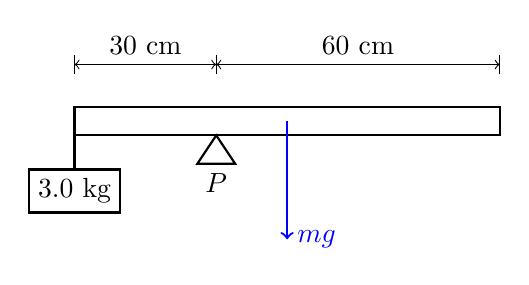
\begin{tikzpicture}[scale=0.6]
	\draw[thick] (-4.5,-.3) rectangle (4.5,.3);
	\draw[thick] (-1.5,-.3) --++ (.4,-.6) --++ (-.8,0) node[midway,below]{$P$} -- cycle;
	\draw[thick,blue,->] (0,0) -- (0,-2.5) node[right]{$mg$};
	\draw[<->] (-4.5,1.2) -- (-1.5,1.2)node[midway,above]{30 cm};
	\draw[<->] (-1.5,1.2) -- (4.5,1.2)node[midway,above]{60 cm};
	\foreach \x in {-4.5,-1.5,4.5} \draw (\x,1) --++ (0,.4);
	\draw[thick] (-4.5,0) --++ (0,-1) node[below, rectangle,draw]{3.0 kg};
	\end{tikzpicture}
	\vspace*{0pt}
\end{wrapfigure}

\example{A uniform rod of length 90 cm is pivoted 30 cm from one end. It is balanced with a 3.0 kg load. Find the mass of the rod.}

\sol take moments about $P$:

{
	\centering
	
	$ 3.0 \times 9.81 \times 0.30 = m \times 9.81 \times \left(0.60-\frac{1}{2}\times0.90\right)$
	
}

so we find mass of rod: $m = 1.5 \text{ kg}$ \eoe


\example{A student balances a metre rule of mass 120 g supported on a fulcrum at the 40 cm mark. She then places a 20 g mass on the 70 cm mark and a 50 g mass on the 25 cm mark as shown. To balance the rule, what mass should she place on the 15 cm mark?}

\begin{figure}[ht]
	\centering
	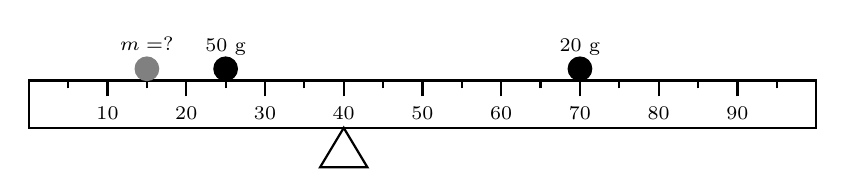
\begin{tikzpicture}[scale=1]
	\draw[thick] (-5,-.3) rectangle (5,.3);
	\foreach \x in {10,20,...,90} \draw[thick] (\x/10-5,.1) node[below]{{\scriptsize \x}} --++ (0,.2) ; 
	\foreach \x in {5,15,...,95} \draw[thick] (\x/10-5,.2) --++ (0,.1) ; 
	\draw[thick] (-1,-.3) --++ (.3,-.5) --++ (-.6,0) -- cycle;
	\draw[fill] (2,.45) circle (0.15);
	\node[above] at (2,.5) {{\scriptsize 20 g}};
	\draw[fill] (-2.5,.45) circle (0.15);
	\node[above] at (-2.5,.5) {{\scriptsize 50 g}};
	\draw[gray,fill] (-3.5,.45) circle (0.15);
	\node[above] at (-3.5,.56) {{\scriptsize $m=?$}};
	\end{tikzpicture}
\end{figure}

\sol take moments about the support:
\begin{equation*}
	mg \times (40-15) + 0.050g\times(40-25) = 0.12g\times(50-40) + 0.020g\times(70-40) \RA m=42 \text{ g} \teoe
\end{equation*}

\example{A cylinder of weight 100 N and diameter 50 cm rests against point $P$ of a curb of height 10 cm. What is the minimum force required to cause the cylinder to roll to the left?}

\begin{wrapfigure}{r}{0.48\textwidth}
	\vspace*{-15pt}
	\centering
	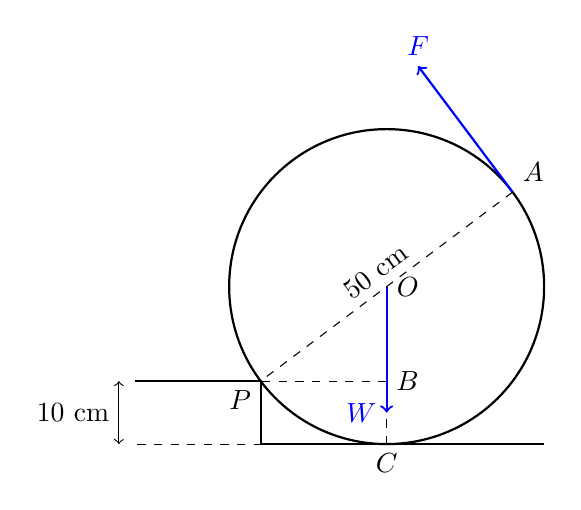
\begin{tikzpicture}[scale=0.4]
	\draw[thick] (0,0) circle (5) node[right]{$O$};
	\draw[thick] (-8,-3) -- (-4,-3) -- (-4,-5) --++ (9,0);
	\draw[thick,blue,->] (4,3) node[above right, black]{$A$} --++ (-3,4) node[above]{$F$};
	\draw[dashed] (4,3) -- (-4,-3) node[midway, above,rotate=36.87] {50 cm};
	\draw[dashed] (0,-3) node[right] {$B$}-- (-4,-3) node[below left] {$P$};
	\draw[dashed] (0,0) -- (0,-5) node[below] {$C$} -- (-8,-5);
	\draw[thick,blue,->] (0,0) -- (0,-4) node[left]{$W$};
	\draw[<->] (-8.5,-3) -- (-8.5,-5) node[midway, left] {10 cm};
	\end{tikzpicture}
	\vspace*{-0pt}
\end{wrapfigure}


\sol to roll the cylinder, force applied must produce a torque no less than that of weight

force is minimum if lever arm is greatest

take moments about $P$ (see diagram):

{
	\centering
	
	$ F_\tmin \times |PA| = W \times |PB| $
	
}

note that $|PB| = \sqrt{|OP|^2 - |OB|^2}$, so

{
	\centering
	
	$|PB| = \sqrt{0.25^2 - (0.25-0.10)^2} = 0.20 \text{ m} $
	
}

plug back into the equation above:
\begin{equation*}
	F_\tmin \times 0.50 = 100 \times 0.20 \RA F_\tmin = 40 \text{ N} \teoe
\end{equation*}

\subsubsection{mechanical equilibrium}

combining Newton's first law and principle of moments, we have the following statement:

\begin{ilight}
	for any mechanical system in equilibrium, two conditions must be satisfied:
	
	\begin{compactenum}
		\item[--] resultant force is zero in any direction: $\sum F = 0$
		
		\item[--] resultant moment is zero about any point: $\sum \tau = 0$
	\end{compactenum}
\end{ilight}

these two conditions allow for many possible equations that can be written down

\begin{wrapfigure}{r}{0.45\textwidth}
	\vspace*{-8pt}
	\centering
	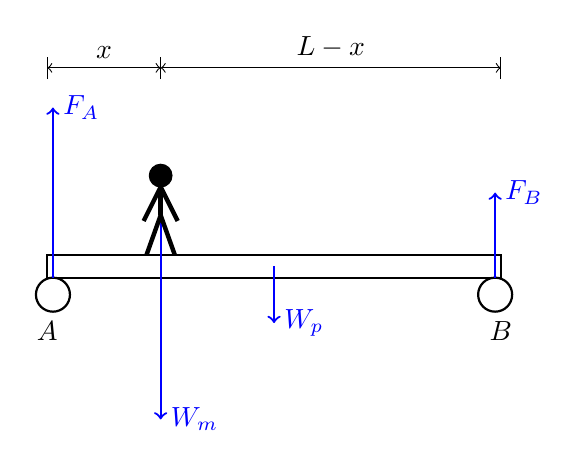
\begin{tikzpicture}[scale=0.72]
	\draw[thick] (-4,-.2) rectangle (4,.2);
	\draw[thick] (-3.9,-.5) circle(.3);
	\draw[thick] (3.9,-.5) circle(.3);
	\draw[thick,blue,->] (0,0) -- (0,-1) node[right]{$W_p$};
	\draw[thick,blue,->] (-2,0.8) --++ (0,-3.5) node[right]{$W_m$};
	\draw[thick,blue,->] (-3.9,-.2) --++ (0,3) node[right]{$F_A$};
	\draw[thick,blue,->] (3.9,-.2) --++ (0,1.5) node[right]{$F_B$};
	\draw[<->] (-4,3.5) -- (-2,3.5)node[midway,above]{$x$};
	\draw[<->] (-2,3.5) -- (4,3.5)node[midway,above]{$L-x$};
	\foreach \x in {-4,-2,4} \draw (\x,3.3) --++ (0,.4);
	\node[below] at (-4,-.8) {$A$};
	\node[below] at (4,-.8) {$B$};
	\draw[fill] (-2,1.6) circle(0.2);
	\draw[ultra thick] (-2,1.5) -- (-2,0.9);
	\draw[ultra thick] (-2,0.9) -- (-2.25,0.2) (-2,0.9) -- (-1.75,0.2);
	\draw[ultra thick] (-2.3,0.8) -- (-2,1.4) -- (-1.7,0.8);
	\end{tikzpicture}
	\vspace*{0pt}
\end{wrapfigure}


\example{A uniform plank of weight 100 N and length $L=6.0 \text{ m}$ rests horizontally on two supports $A$ and $B$. A man of weight 800 N stands a distance of $x=1.5 \text{ m}$ from end $A$. Determine the forces acting at the two supports.}

\sol take moments about $A$: $ W_m x + W_p \cdot\frac{L}{2} = F_B L$

{
	\centering
	
	
	
	$ 800 \times 1.5 + 100 \times 3.0 = F_B \times 6.0 \ra F_B = 250 \text{ N} $
	
}

take moments about $B$: $ W_m (L-x) + W_p \frac{L}{2} = F_A L$

{
	\centering
	
	
	
	$ 800 \times 4.5 + 100 \times 3.0 = F_A \times 6.0 \ra F_B = 650 \text{ N} $
	
}

one can check that: $F_A + F_B = W_m + W_p$, there must be no resultant force in vertical direction \eoe

\newpage


\begin{wrapfigure}{r}{0.4\textwidth}
	\vspace*{0pt}
	\centering
	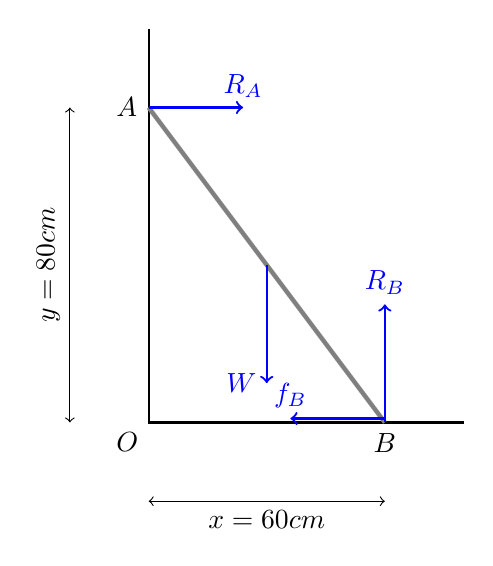
\begin{tikzpicture}[scale=1]
	\draw[thick] (0,5) -- (0,0) node[below left]{$O$} -- (4,0);
	\draw[ultra thick, gray] (0,4) node[left,black]{$A$} -- (3,0) node[below,black]{$B$};
	\draw[<->] (-1,0) -- (-1,4) node[above,midway,rotate=90]{$y=80\text{ cm}$};
	\draw[<->] (0,-1) -- (3,-1) node[below,midway]{$x=60\text{ cm}$};
	\draw[thick,blue,->] (0,4) --++ (1.2,0) node[above]{$R_A$};
	\draw[thick,blue,->] (3,0) --++ (0,1.5) node[above]{$R_B$};
	\draw[thick,blue,->] (3,0.05) --++ (-1.2,0) node[above]{$f_B$};
	\draw[thick,blue,->] (1.5,2) --++ (0,-1.5) node[left]{$W$};
	\end{tikzpicture}
	\vspace*{-16pt}
\end{wrapfigure}


\example{A uniform ladder of weight 120 N rests on a rough ground against a smooth wall as shown. The dimensions are labelled on the diagram. (a) What is the contact force acting at $B$? (b) What is the contact force acting at $A$? (c) What is the frictional force at $B$?}


\sol we draw free-body diagram as shown

resolve vertically: $R_B = W \RA R_B = 120 \text{ N}$

take moments about $B$: $R_A y = W \frac{x}{2}$

{
	\centering
	
	$ R_A = \frac{120 \times 0.30}{0.80} = 45 \text{ N}$
	
}

resolve horizontally: $f_B = R_A \RA f_B = 45 \text{ N}$ \eoe

\begin{wrapfigure}{r}{0.42\textwidth}
	\centering
	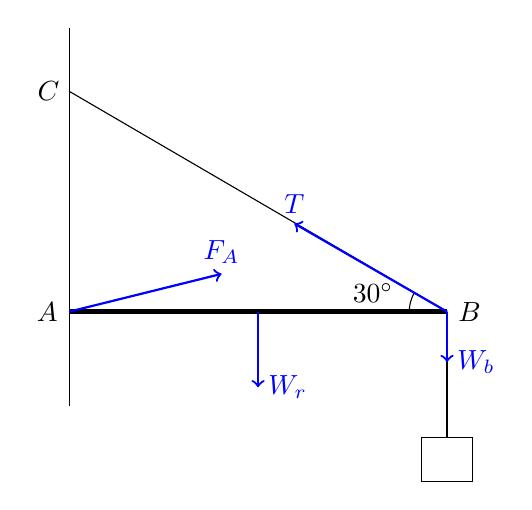
\begin{tikzpicture}[scale=0.8]
	\draw (0,-1.5) -- (0,4.5);
	\draw[ultra thick] (0,0) node[left]{$A$} -- (6,0) node[right]{$B$};
	\draw (6,0) -- (0,3.5) node[left]{$C$};
	\draw (5.4,0) arc(180:150:0.6);
	\node[left] at (5.3,0.3) {$30^\circ$};
	\draw (6,0) -- (6,-2);
	\draw (5.6,-2.7) rectangle (6.4,-2);
	\draw[thick,blue,->] (6,0) --++ (0,-0.8)node[right]{$W_b$};
	\draw[thick,blue,->] (3,0) --++ (0,-1.2)node[right]{$W_r$};
	\draw[thick,blue,->] (6,0) --++ (150:2.8)node[above]{$T$};
	\draw[thick,blue,->] (0,0) --++ (12.1*.2,3*.2)node[above]{$F_A$};
	\end{tikzpicture}
	\vspace*{-20pt}
\end{wrapfigure}


\example{The diagram shows a uniform rod $AB$ of weight 60 N that is held horizontally to a vertical wall by means of a light string. The string is attached to the rod at $B$, where a basket of weight 40 N is suspended. The other end of the string is fixed on the wall at $C$. The angle between the string and the rod is $30^\circ$. (a) Find the tension in the string. (b) Find the force acting on the rod at $A$.}

\sol take moments about $A$: $TL\sin\theta = W_b L + W_r  \frac{1}{2}L$

{
	\centering
	
	$ T \sin30^\circ = 40 + 60\times\frac{1}{2} \RA T=140 \text{ N} $
	
}

resolve horizontally: $F_{A,x} = T\cos\theta \RA F_{A_x}=140\cos30^\circ \approx 121 \text{ N}$

resolve vertically: $F_{A,y}+T\sin\theta = W_r + W_b \RA F_{A,y} = 60+40 - 140\sin30^\circ = 30 \text{ N} $

force at $A$: $F_A = \sqrt{F_{A,x}^2 + F_{A,y}^2} \RA F_A = \sqrt{121^2 + 30^2} \approx 125 \text{ N}$ \eoe


\subsection{two forces in equilibrium}

the problem of two balanced forces is trivial

\begin{wrapfigure}{R}{0.2\textwidth}
	\vspace{-15pt}
	\begin{center}
		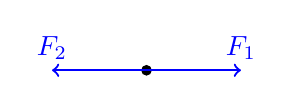
\begin{tikzpicture}[scale=0.6]
		\draw[fill] (0,0) circle(0.1);
		\draw[thick,blue,->] (0,0) -- (2,0) node[above]{$F_1$};
		\draw[thick,blue,->] (0,0) -- (-2,0) node[above]{$F_2$};
		\end{tikzpicture}
	\end{center}
	\vspace{-10pt}
\end{wrapfigure}

suppose two forces $F_1$ and $F_2$ are acting on an object in equilibrium

\begin{compactenum}
	\item[--] to have zero resultant force, $F_1$ and $F_2$ must be equal but opposite
	
	\item[--] to have zero resultant moment, $F_1$ and $F_2$ must act along same line
	
	otherwise they would produce torque of couple, which causes turning effects
\end{compactenum}


\subsection{three forces in equilibrium}

\subsubsection{force triangle}

when there are more than two forces, situation becomes more complicated

one can use \emph{vector diagram} to solve the problem

suppose a set of forces $\overrightarrow{F_1}$, $\overrightarrow{F_2}$, $\cdots$, $\overrightarrow{F_n}$ are in equilibrium

no resultant force requires $\overrightarrow{F_1} + \overrightarrow{F_2} + \cdots + \overrightarrow{F_n} = 0$

recall that resultant force is vector sum of all forces acting, and now this sum has to vanish, so if the force vectors are connected head to tail, they should form a closed $n$-polygon

\begin{figure}[ht]
	\centering
	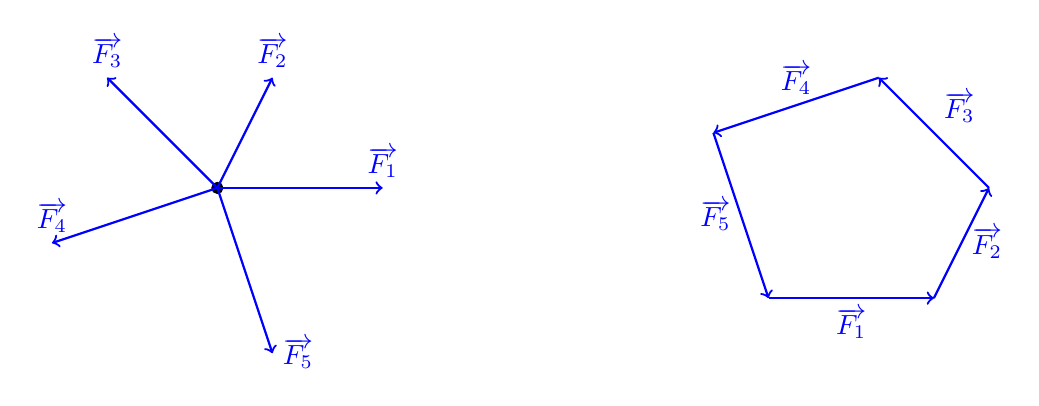
\begin{tikzpicture}[scale=0.7]
	\draw[fill] (0,0) circle(0.1);
	\draw[thick,blue,->] (0,0) -- (3,0) node[above]{$\overrightarrow{F_1}$};
	\draw[thick,blue,->] (0,0) -- (1,2) node[above]{$\overrightarrow{F_2}$};
	\draw[thick,blue,->] (0,0) -- (-2,2) node[above]{$\overrightarrow{F_3}$};
	\draw[thick,blue,->] (0,0) -- (-3,-1) node[above]{$\overrightarrow{F_4}$};
	\draw[thick,blue,->] (0,0) -- (1,-3) node[right]{$\overrightarrow{F_5}$};
	
	\node at (6,0) {\Huge{$\RA$}};
	
	\draw[thick,blue,->] (10,-2) -- ++(3,0) node[midway,below]{$\overrightarrow{F_1}$};
	\draw[thick,blue,->] (13,-2)-- ++(1,2) node[midway,right]{$\overrightarrow{F_2}$};
	\draw[thick,blue,->] (14,0)-- ++(-2,2) node[midway,above right]{$\overrightarrow{F_3}$};
	\draw[thick,blue,->] (12,2)-- ++(-3,-1) node[midway,above]{$\overrightarrow{F_4}$};
	\draw[thick,blue,->] (9,1) -- ++(1,-3) node[midway,left]{$\overrightarrow{F_5}$};
	\end{tikzpicture}
	\caption*{an $n$-polygon formed by a set of $n$ balanced forces}\label{fig:force-polygon}
\end{figure}

in the case of three balanced forces, net force is zero means they should form a \keypoint{force triangle}

unknown forces can then be solved by cracking a geometric problem

\begin{wrapfigure}{r}{0.33\textwidth}
	\vspace*{-16pt}
	\centering
	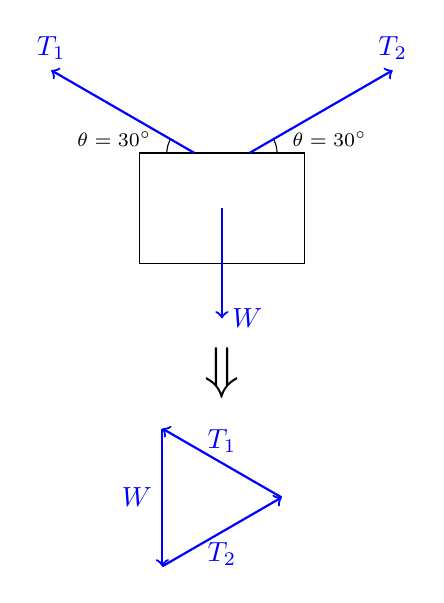
\begin{tikzpicture}[scale=0.7]
	\draw (-1.5,0) rectangle (1.5,-2);
	\draw[->,thick,blue] (0,-1) -- (0,-3) node[right]{$W$};
	\draw[->,thick,blue] (-0.5,0) -- ++(150:3) node[above]{$T_1$};
	\draw (-1,0) arc(180:150:0.5);
	\node[left] at (-1.1,0.25) {\scriptsize$\theta=30^\circ$};
	\draw (1,0) arc(0:30:0.5);
	\node[right] at (1.1,0.25) {\scriptsize$\theta=30^\circ$};
	\draw[->,thick,blue] (0.5,0) -- ++(30:3) node[above]{$T_2$};
	\node at (0,-4) {\huge{$\Downarrow$}};
	\draw[->,,thick,blue] (-1.0825,-5) -- ++(0,-2.5) node[midway,left]{$W$};
	\draw[->,,thick,blue] (-1.0825,-7.5) -- ++(30:2.5) node[midway,below]{$T_2$};
	\draw[<-,,thick,blue] (-1.0825,-5) -- ++(-30:2.5) node[midway,above]{$T_1$};
	\end{tikzpicture}
	\vspace*{-10pt}
\end{wrapfigure}

\example{A painting of weight $W=20\text{ N}$ is supported by two strings as shown. Both strings form an angle $\theta=30^\circ$ to the horizontal. Find the tension in the strings.}



\sol by resolving forces, we have: 

{
	\centering
	
	$\Biggl\{\begin{array}{l}
	T_1 \cos\theta = T_2 \cos\theta\\
	T_1\sin\theta + T_2\sin\theta = W
	\end{array} $ 
	
}

we solve the equations to obtain:

{
	\centering
	
	$ T_1 = T_2  = \frac{W}{2\sin\theta} = \frac{20}{2\sin30^\circ}=20\text{ N} $
	
}


alternatively, we can construct the force triangle as shown

$T_1$, $T_2$ and $W$ form an equilateral triangle, so
\begin{equation*}
	T_1=T_2=W=20\text{ N} \teoe
\end{equation*}





\newpage

\begin{wrapfigure}{r}{0.33\textwidth}
	\vspace*{-5pt}
	\centering
	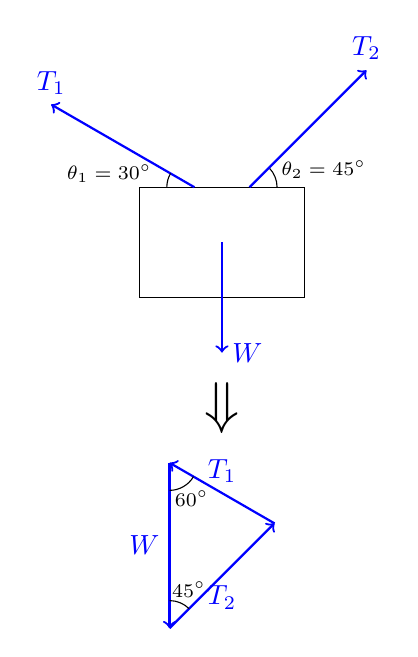
\begin{tikzpicture}[scale=0.7]
	\draw (-1.5,0) rectangle (1.5,-2);
	\draw[->,thick,blue] (0,-1) -- (0,-3) node[right]{$W$};
	\draw[->,thick,blue] (-0.5,0) -- ++(150:3) node[above]{$T_1$};
	\draw (-1,0) arc(180:150:0.5);
	\node[left] at (-1.1,0.25) {\scriptsize$\theta_1=30^\circ$};
	\draw (1,0) arc(0:45:0.5);
	\node[right] at (0.9,0.32) {\scriptsize$\theta_2=45^\circ$};
	\draw[->,thick,blue] (0.5,0) -- ++(45:3) node[above]{$T_2$};
	\node at (0,-4) {\huge{$\Downarrow$}};
	\draw[->,,thick,blue] (-.95,-5) -- ++(0,-3) node[midway,left]{$W$};
	\draw[->,,thick,blue] (-0.95,-8) -- ++(45:2.69) node[midway,below]{$T_2$};
	\draw[<-,,thick,blue] (-.95,-5) -- ++(-30:2.20) node[midway,above]{$T_1$};
	\draw (-0.95,-5.5) arc(-90:-30:0.5);
	\draw (-0.95,-7.5) arc(90:45:0.5);
	\node at (-0.55,-5.65) {{\scriptsize $60^\circ$}};
	\node at (-0.6,-7.3) {{\scriptsize $45^\circ$}};
	\end{tikzpicture}
	\vspace*{-10pt}
\end{wrapfigure}

\example{The same painting of weight $W=20\text{ N}$ is supported by two strings at different angles $\theta_1=30^\circ$ and $\theta_2=45^\circ$ as shown. Find the forces in the two strings.}


\sol by resolving forces, we have: 

{
	\centering
	
	$ \left\{\begin{array}{l}
		T_1 \cos\theta_1 = T_2 \cos\theta_2\\
		T_1\sin\theta_1 + T_2\sin\theta_2 = W
	\end{array} \right.
	\RA
	\left\{\begin{array}{l}
	\frac{\sqrt{3}}{2}T_1 = \frac{\sqrt{2}}{2}T_2\\
	\frac{1}{2}T_1 + \frac{\sqrt{2}}{2}T_2 = 20
	\end{array} \right.
	$
	
}


\eqyskip solving this, we find: $T_1 \approx 14.6\text{ N}\, , \, T_2 \approx 17.9\text{ N} $

alternatively, we construct the force triangle, computation for $T_1$ and $T_2$ would be more straightforward

the three forces are related by the the law of sine:

{
	\centering
	
	$\frac{W}{\sin75^\circ} = \frac{T_1}{\sin45^\circ} = \frac{T_2}{\sin60^\circ} $
	
}

from this we get the same result: $T_1 \approx 14.6\text{ N}\, , \, T_2 \approx 17.9\text{ N} $ \eoe



\subsubsection{concurrent forces}

for three forces in equilibrium, they must produce zero resultant moment about any point

suppose lines of action of $F_1$ and $F_2$ meet at point $P$

moment of $F_1$ and moment of $F_2$ about $P$ are both zero

to produce zero resultant moment about $P$, then moment of $F_3$ about $P$ must vanish

this suggest line of action of $F_3$ must pass through point $P$

therefore lines of action of $F_1$, $F_2$ and $F_3$ must pass through the same point\footnote{In the case of three parallel forces in equilibrium, we can introduce the notion of an ideal point at infinity, so that parallel lines could meet at that point.}

such three forces are said to be \emph{concurrent}

\subsubsection*{summary for three forces in equilibrium}

for three forces in equilibrium, we can now conclude:

\begin{compactenum}
	\item[--] the three force vectors must be able to form a force triangle
	
	this is a consequence of zero resultant force
	
	\item[--] the lines of action for the three forces must pass through same point
	
	this is a consequence of zero resultant moment
\end{compactenum}





\ifthenelse{\includequestions=1}{
	
\subsection{end-of-chapter questions}


\subsubsection*{mechanical equilibrium}

\question{Is it possible for an object to be in equilibrium if only one force is acting on it?}

\question{If three forces are in equilibrium, suggest and explain whether the lines of action must lie in the same plane.}

}{}